\chapter{Methods}
\label{sec:methods}
In this work, a novel approach for an end-to-end application for explicit surface 
reconstruction from unstructured point cloud data is proposed, based on a graph convolutional network (~GCN~) by Wang et al. \cite{wang2018pixel2mesh}, transforming images 
to polygonal meshes. It is heavily modified to allow point cloud data as input, though still able to infer polygonal meshes from previously unseen datapoints. 
This chapter outlines the changes made to the network by Wang et al. , new extensions 
for learning in three-dimensional space on point cloud data, and its variations to
 yield the best possible results. 
The proposed network ~(~ \emph{points2mesh} ~) learns feature vectors from point cloud data with their
 normal orientation, which are utilized to deform an initial polygonal 
 mesh object, like an ellipsoid, resulting in an approximation of a mesh, based on the input point cloud.

Section \ref{networkconfig} specifies the network's structure as well as
 proper objective functions in detail which operate the two-part
  convolutional network.

Subsequentially, section \ref{dataset} specifies the dataset used to
 train the networks, as well as how it was designed and constructed.

\section{Neural network structure}
\label{networkconfig}
Choosing suitable configurations, proper hyperparameters tunings,
 or even an appropriate dataset for a neural network is not a clear-cut decision. 
 Thus, several configurations and hyperparameter tunings have been developed.
  Subsection \ref{generalsystem} first describes the general idea of the neural network, followed by a detailed
   break down of its structure and configurations in section \ref{fconv} and \ref{gcnconv} ,
   Subsequentially, a closer look at utilized objective functions in subsections \ref{lossfuncs} will be taken.
   Finally, every considered configuration of the neural network is outlined in subsection \ref{configurations}.
\subsection{General system overview}
\label{generalsystem}

\begin{figure}
   \begin{center}
   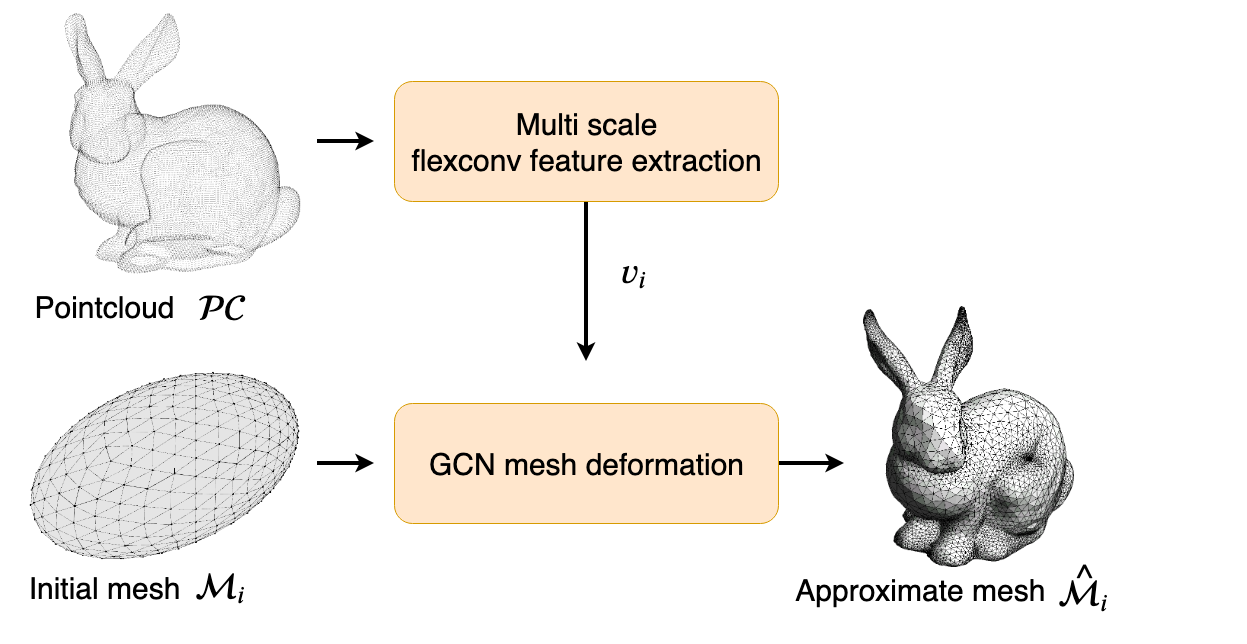
\includegraphics[width=15cm]{general_structure}
   \caption{\todo{general network config explanation}}
   \label{fig:generalconfig}
   \end{center}
 \end{figure}
 The general goal of the neural network $\mathcal{N}_{recon}$ is to provide an end-to-end solution for 
 explicit surface reconstruction given a collection of unstructured point cloud data ~(~$\mathcal{PC}$~) in three-dimensional 
 space with their normal orientation $\textbf{n}_{x_i}$. 

 With:
 \begin{align}
      \forall \textbf{x}_i \in \mathcal{PC} : 
      \textbf{x}_i =
      \begin{bmatrix}
            x \\
            y\\
            z
          \end{bmatrix} \in [-1,1]^3
   \end{align}

 Overall, the network structure is separated into two distinct parts,
  each with its specific purpose to fulfill. As seen in Figure \ref{fig:generalconfig}, the neural 
  network $\mathcal{N}_{recon}$ gets two different inputs, whereas each input is processed in a different part of the network.
 First, the input data $\mathcal{PC}$ is fed into the upper half of the network, called \emph{flexconv feature extraction}
  $\mathcal{N}_{flex}$ ~(~ See Figure \ref{fig:generalconfig} ~). In a multiscale convolutional operation,
   a collection of feature vectors $v_{x_n}$ is extracted, 
which is fed into the lower part of the network.

  The second part, as seen in the lower half of figure \ref{fig:generalconfig}, illustrates 
  a \emph{graph convolutional network} $\mathcal{N}_{gcn}$. Given an initial ellipsoid
  polygonal mesh $\mathcal{M}_{e}$, $\mathcal{N}_{gcn}$ deforms it, estimating $\hat{\mathcal{M}}$.
   Where $\hat{\mathcal{M}}$ is the best matching estimate for the ground truth mesh $\mathcal{M}_{gt}$ given $\mathcal{PC}$.
   The deformation process is assisted by supplying feature vectors $v_{x_n}$ from $\mathcal{N}_{flex}$, also adding more
    vertices to the initial ellipsoid $\mathcal{M}_{e}$ in three steps during the deformation process.
\subsection{Flexconv feature extraction}
\label{fconv}

\begin{figure}
   \begin{center}
   \includegraphics[width=14cm]{flexconv}
   \caption{\todo{only flexconvpart}}
   \label{fig:flexconv}
   \end{center}
 \end{figure}

In traditional convolutional networks in context of computer graphics, the data at hand is often given as two dimensional images.
 In the case of three-dimensional processing, structured 3D grids are then a popular tool for natural processing 
 of such. However, since converting data from $\mathcal{PC}$ to a voxelized representation diminished its resolution, 
 it is now kept as its unstructured base form of point cloud data. 

As seen in the upper half of figure \ref{fig:flexconv}, $\mathcal{N}_{flex}$ processes $\mathcal{PC}$ to compute
 a collection of three feature vectors $v_{x_n}$ on a multiscale measure, working as follows.
 The network $\mathcal{N}_{flex}$ takes a vector of three-dimensional points $\textbf{x}_i \in \mathcal{PC}$ 
 of size $[3,1024]$ or $[3,8000]$ ~(~depending on the configuration ~), assigning each point its own 3D coordinates
  as his current feature $v_i$.
Then, it is separated into three consecutive parts, where each section $\mathcal{S}$ processes the point cloud vector $\textbf{x}_i$ and features $\textbf{v}_i$
 with two consecutive flexconv operators and a flexpool operator while expanding the dimension by a factor of $32$ in each section.
After convolving, the point cloud is sampled down by a factor of four each time by weighted reservoir sampling~(~wrs~)~. 
Following every convolution, the coordinates $\textbf{x}_i$ and their features $\textbf{v}_i$ are collected. 
This compiles the multiscale feature vector $v_i^s$, which consits of key points in $\mathcal{PC}$ needed for the deformation steps in the second part of the network.



\subsection{GCN mesh deformation}
   \label{gcnconv}
   \begin{figure}
      \begin{center}
      \includegraphics[width=14cm]{gcnpart}
      \caption{\todo{only gcn}}
      \label{fig:gcn}
      \end{center}
   \end{figure}
   As for the second part of the network $\mathcal{N}_{recon}$, it consists 
   of a graph convolutional network $\mathcal{N}_{gcn}$, taking a basic polygonal 
   shape $\mathcal{M}_{i}$ as input, for example an ellipsoid form.
   The input mesh can directly be transformed into a graph structure, which the \emph{gcn}
   can process since each vertex in the mesh corresponds to a node in the graph.Its structure, i.e., 
   the number of vertices and edges, has to be known beforehand.
   Moreover, the same is true for the correspondence of edges in the mesh and edges in the graph. Thus, $\mathcal{M}_{i}=\mathcal{G}(V,E)$,
   with $V$ being the vertices in the graph, and $E$ the set of edges, connecting $V$.
   Furthermore, similarly to \ref{fconv}, the three-dimensional coordinates of each vertex in
   the initial mesh are utilized as feature vectors $f_i$ for $\mathcal{G}(V,E,f_i)$. Since $\mathcal{M}_{i}$ corresponds to $\mathcal{G}$, 
   in the following sections, the input graph $\mathcal{G}$ of $\mathcal{N}_{gcn}$ is still referenced as input mesh $\mathcal{M}_{i}$.
 
   $\mathcal{N}_{gcn}$ is separated into three parts, as seen in figure \ref{fig:gcn}.
   The primary process of one such segment consists of convolving on the graph for a set
   amount of iterations. Then, information from feature vectors $\textbf{v}_i$ from $\mathcal{N}_{flex}$ 
   to local feature vectors of the graph $f_i = [f_i,\textbf{v}_i]$ are appended by projecting them
   from the point cloud data onto the graph. Subsequently, the graph's vertices and edges are increased 
   with a specialized \emph{unpooling operation}. $\mathcal{N}_{gcn}$ repeats this process two more times 
   to compute $\hat{\mathcal{M}}$, approximating the underlying surface information for the input $\mathcal{PC}$.

   \label{gcnconv}
   \begin{figure}
      \begin{center}
      \includegraphics[width=10cm]{unpool}
      \caption{\todo{unpool}}
      \label{fig:unpool}
      \end{center}
    \end{figure}

   The graph convolutional network is limited to a rigid structure of graphs on which it operates. 
   Thus, it is necessary to define it before starting to train the network. Theoretically, it is possible 
   to train the complete reconstruction with $\mathcal{N}_{recon}$ on an already highly detailed graph with 
   many edges and vertices. However, such a graph is harder to deform in a correct way to approximate $\hat{\mathcal{M}}$, 
   since it has many more trainable variables and thus may take much longer to converge, if at all. Hence, it would be easier to
   first deform an initial mesh with a low amount of detail, then increase its detail level over and over, deform anew, until it converges.
   Wang et al. \cite{wang2018pixel2mesh} describe an \emph{unpooling layer}, which enables $\mathcal{M}_i$ to gain more detail,
    every time it is applied to it (~$\mathcal{M}_0 \cdots \mathcal{M}_2$~). 
   This edge-based unpooling layer adds a new edge in the midpoint of each neighboring edge for the graph $\mathcal{G}$ as seen in 
   figure \ref{fig:unpool}. Subsequently, it connects the new ones, for that the amount of neighbors for each vertex stays the same. 
   Though, the structure of the resulting graphs has to be known as well. Otherwise stable training of $\mathcal{N}_{gcn}$ would not be possible. 
   $\mathcal{N}_{gcn}$ utilizes the layer twice, each time after deforming the current state of the graph and projecting $v_i$ 
   from the $\mathcal{PC}$ onto $\mathcal{M}_{i}$. 

   \begin{figure}
      \begin{center}
      \includegraphics[width=6cm]{align}
      \includegraphics[width=6cm]{no_align}
      \caption{\todo{graph alignment, unbiased left, biased}}
      \label{fig:align}
      \end{center}
   \end{figure}

   
   Since the data in $\mathcal{PC}$, may not always be uniformly sampled ~(~See section \ref{dataset}~),
   it is essential to compensate for the positional bias of the $\mathcal{PC}$ in relation to $\mathcal{M}_{i}$ as seen in figure \ref{fig:align}. 
   $\mathcal{N}_{gcn}$ begins with a \textbf{graph alignment layer} , moving the arithmetic midpoint of the graph $\mathcal{M}_{i}$ 
   on top of the arithmetic midpoint of $\textbf{x}_i \in \mathcal{PC}$:
   \begin{align}
   \label{form:align}
   \forall \textbf{x}_{gcn} \in \mathcal{M}_i : \textbf{x}'_{gcn} = \textbf{x}_{gcn} + 
   (\frac{1}{|\mathcal{PC}|}\sum_{x_i \in \mathcal{PC}}x_i - \frac{1}{|\mathcal{M}_{i}|}\sum_{x_{gcn} \in \mathcal{M}_i}x_{gcn})
   \end{align}
   After repositioning the graph, it is rescaled to the value domain of $[-1,1]^3$, if it exceeds it.
   Besides, this facilitates learning a more generalized form for deforming the mesh, for that $\mathcal{N}_{gcn}$ can not rely on absolut but rather relative positioning of $\mathcal{M}_{i}$ during 
   convolution.

   \subsubsection*{Feature projection}
   \label{featureproj}
   \begin{figure}
      \begin{center}
      \includegraphics[width=5cm]{projection}
      \caption{\todo{graph projection}}
      \label{fig:proj}
      \end{center}
   \end{figure}

   Considering only \emph{convolutional operations}, \emph{graph alignment layer} and \emph{unpooling layer}
   of $\mathcal{N}_{gcn}$, a connection from $\mathcal{N}_{flex}$ has yet to be made. Ideally, a 
   correlation between $\mathcal{PC}$ and $\mathcal{M}_{i}$ is created. The goal of $\mathcal{N}_{gcn}$ is 
   to deform $\mathcal{M}_{i}$ based on learned feature vectors $\textbf{v}_i$ from $\mathcal{N}_{flex}$. 
   Mathematically by default, no direct correlation between these two exist. Thus, the 
   \emph{feature projection layer} is proposed. It assigns for each vertex in $\mathcal{M}_i$,
   features from $\mathcal{N}_{flex}$ based on the distance from $\mathcal{M}_{i}$ to their $k$-nearest 
   neighbors in $\mathcal{PC}$. 

   As seen in blue in figure \ref{fig:proj}, every point in $\mathcal{PC}$ resides in the same coordinate
   system as vertices $p_j \in \mathcal{M}(V,E)$ ~(~ Illustrated as green points with their connecting vertices in black ~).
   For each vertex $p_j$, the \emph{feature projection layer} computes the $k$-nearest neighbors in $\mathcal{PC}$ 
   ~(~Here $k=6$ ~). Higher values for $k$ compensate for unstable performance of nearest neighbor search, 
   while lower values speed up excecution and thus training time.
   Features $[\textbf{v}_n^s,\cdots,\textbf{v}_{n+k}^s]$ of points $[\textbf{x}_{n}^s,\cdots,\textbf{x}_{n+k}^s]$ are scaled by 
   the distances $d_i = |\textbf{x}_i  - p_j|$.
   The final feature vector $f_i$ assigned to $p_i$ is calculated like the following:
   \begin{align}
      \forall p_j \in \mathcal{M}_{i} : f_i^s &= \frac{1}{k}\sum_{\forall x_i^s \in knn(p_j),s\in \mathcal{S}} \frac{v_i^s}{1 + |x_i^s-p_j|^2}
   \end{align}
   Where $v_i$ is the respective feature vector stored at point $\textbf{x}_i^s$. This is repeated for each scaling $s$ in $\mathcal{S}$ of 
   $\mathcal{N}_{flex}$ where a feature vector is propagated out of the subnetwork ~(~ See figure \ref{fig:flexconv}~).

\subsection{Loss functions}
\label{lossfuncs}s
   The losses are defined based on the network of Wang et al. \cite{wang2018pixel2mesh}, 
   and adapted accordingly to work with point cloud based input data. Given $\textbf{x}_i$ 
   and normal orientation $\textbf{n}_i$, an objective function $\mathcal{F}$ is defined as 
   follows to help generate good-looking results.

   A symmetrical \emph{chamfer distance loss} $l_{ch}$ tries to ensure that vertices of $\mathcal{M}_{i}$ 
   are located close to other points $\textbf{x}_i$ in ground truth data $\mathcal{PC}$. It sums
   up for each vertex $p_j\in \mathcal{M}_i$ the distance to its nearest neighbor in $\mathcal{PC}$
   and for each point $\textbf{x}_i\in \mathcal{PC}$ the distance to its nearest neighbor in
   $\mathcal{M}_i$. Though, it is scaled by sizes of $|\textbf{x}_i|$ relative to $|p_j|$, depending on how often 
   $\mathcal{M}_i$ already has been unpooled (~See Appendix \ref{sec:appendix} for their formula~).

   Furthermore, Wang et al. propose an edge length loss $l_{edge}$ in $\mathcal{F}$ , reducing the overall mean of lengths of the edges.
   And scaling it up by a predetermined constant value of $300$, as seen in formula \ref{form:edge}. 
   Only considering $l_{ch}$ and $l_{edge}$ ignores the orientation of neighboring faces.
   Wang et al.'s $l_{cos}$ term guides $\mathcal{F}$ to orientate neighboring edges towards the 
   same direction since most real meshes have smooth surfaces. This approximating term is illustrated in formula \ref{form:cos}.
   Additionally, since $l_{ch},l_{edge},l_{cos}$ may still lead to optimizations which gravitate towards local minima, they introduce 
   a laplacian regularizer $l_{lap}$ which avoids self intersecting meshes and moving single vertices too freely during
    the deformation process (~See Appendix \ref{sec:appendix} for their formula~).
   \begin{align}
      \label{form:edge}
      l_{edge} &= \frac{300}{|E|}\sum_{e\in E}||e||^2\\
      \label{form:cos}
      l_{cos} &= \frac{1}{2|E|}\sum_{e\in E}normal(e) \cdot e
   \end{align}


   In most extreme cases, it is possible for different, not neighboring vertices to land on top on each other, or close to each other 
   with distances $< \epsilon$. Since this case is not covered by avoiding selfintersections with the laplacian regularizer, a 
   \emph{collapse loss} $l_{col}$ is included in $\mathcal{F}$, defined as:
   \begin{align}
      l_{col} &= \frac{1}{|\mathcal{M}_{i}|}\sum_{ nn(p_j)-p_j > \epsilon,\forall p_j \in \mathcal{M}_{i}} 1
   \end{align}

   $\mathcal{N}_{recon}$ optimizes against the objective function $\mathcal{F}=l_{ch}+l_{col}+l_{cos}+l_{edge}$
    to obtain an approximate mesh $\hat{\mathcal{M}}$ which characterizes $\mathcal{PC}$.

\subsection{Network configurations $\mathcal{C}$}
\label{configurations}
Finding suitable hyperparameters and an appropriate network structure 
is no easy task. Tuning hyperparameters in small increments, removing or including 
more layers in either $\mathcal{N}_{recon}$ or $\mathcal{N}_{flex}$ may change results drastically.
 Therefore, some configurations have advantages over other 
configuration, while still having disadvantages in other aspects.
Thus, several configurations have been carved out and are specified 
in detail later evaluation. This section illustrates how the configurations deviate from the general
 network structure presented in section \ref{generalsystem} through \ref{gcnconv}.
Though, every configuration uses an ellipsoid triangle/quad mesh $\mathcal{M}_{i}$ with $156$ vertices for the deformation process of $\mathcal{N}_{gcn}$.
Consecutive \emph{unpooling} operations increase the count to $618$, and finally to $2466$ vertices.

\textbf{$\mathcal{C}_1$: Baseconfiguration}
\begin{figure}
   \begin{center}
   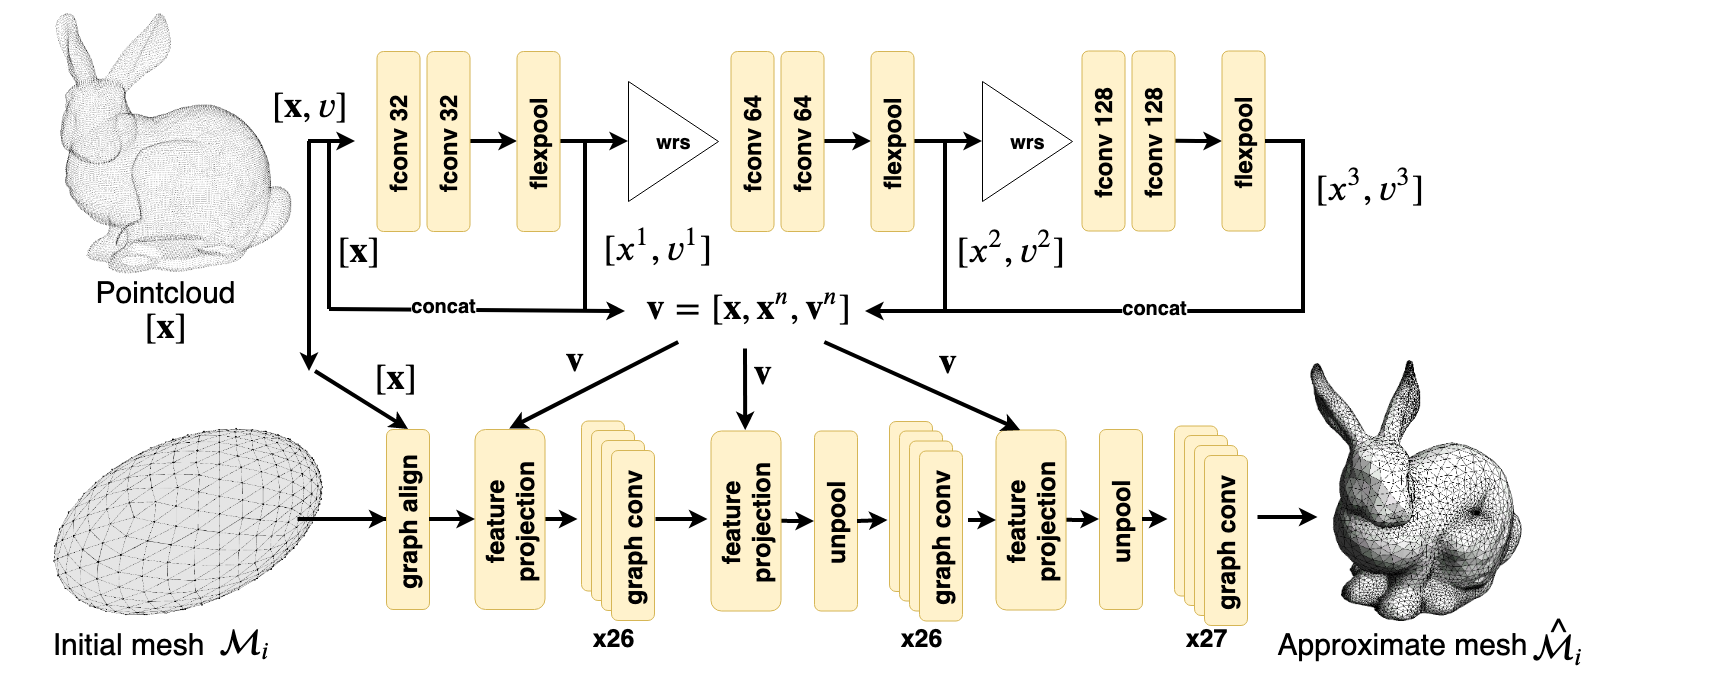
\includegraphics[width=14cm]{c1}
   \caption{\todo{c1 description}}
   \label{fig:c1}
   \end{center}
\end{figure}
Configuration $\mathcal{C}_1$, as described in this chapter and seen in figure \ref{fig:c1},
 illustrates the base structure of $\mathcal{N}_{recon}$.
It is trained on an input $\mathcal{PC}$ with $1024$ as well as $800$ samples and increases
 the detail of $\mathcal{M}_{i}$ twice. 

\textbf{$\mathcal{C}_2$: High detailed baseconfiguration}
\begin{figure}
   \begin{center}
   \includegraphics[width=14cm]{c2}
   \caption{\todo{c2 description}}
   \label{fig:c2}
   \end{center}
\end{figure}
Configuration $\mathcal{C}_2$ corresponds to $\mathcal{C}_1$ almost identically, 
with the exception of increasing the count of \emph{unpooling layer} from two to three, thus increasing
 the number of vertices to 10626. As seen in figure \ref{fig:c2} marked as green layer components, $\mathcal{N}_{gcn}$
  is expanded by appending another \emph{projection} and  \emph{unpooling} layer, as well
   as a \emph{convolution} block at the end. Similarly $\mathcal{C}_2$ is trained with $1024$ as well as $800$ samples
   in $\mathcal{PC}$.

\textbf{$\mathcal{C}_3$: Biased neighbor features}

Configuration $\mathcal{C}_3$, similarly configured like $\mathcal{C}_1$, but with a difference in the implementation of the \emph{projection layer}.
Instead of only projecting feature vectors $v_i$ of $\mathcal{PC}$ onto the mesh, it also adds the mean vector $\textbf{x}_i$ 
to the final feature vector $f_i^s$ for $\mathcal{M}_i$.
 \begin{align}
      \forall p_j \in \mathcal{M}_{i} : y_i^s &= \frac{1}{k}\sum_{\forall x_i^s \in knn(p_j),s\in \mathcal{S}} \frac{x_i^s}{1 + |x_i^s-p_j|^2}
   \end{align}
Thus, $\mathcal{N}_{gcn}$ utilizes the following feature vector $f_i$ after projecting in each detail step of the mesh $\mathcal{M}_i$:
\[f_i = [f_i, y_i^1, v_i^1, y_i^2, v_i^2,y_i^3, v_i^3,] \]
Additionally, as a variation of $\mathcal{C}_3$, the first layer of $\mathcal{N}_{gcn}$, the \emph{graph alignment layer} is omitted and 
thus defining configuration $\mathcal{C}'_3$. Removing the layer introduces a positional bias of the initial shape $\mathcal{M}_i$ into the network, but
leads to interesting reconstructions worthy of evaluating in more detail.

\textbf{$\mathcal{C}_4$: Compact GCN with simple projection}
\begin{figure}
   \begin{center}
   \includegraphics[width=14cm]{c4}
   \caption{\todo{c4 description}}
   \label{fig:c4}
   \end{center}
\end{figure}
Finally, configuration $\mathcal{C}_4$ reduces the amount of convolutional layers in $\mathcal{N}_{gcn}$ as seen in figure \ref{fig:c4}.
Furthermore, the distance based falloff $\frac{1}{1+d}$ in the \emph{projection layer} is excluded, 
while also computing only one nearest neighbor, $k=1$ in that particular layer. 

\section{Dataset}
\label{dataset}
   Finding and designing a suitable dataset $\mathcal{D}$
   to train the network on is just as crucial as designing its structure. 
   Such a suitable dataset is \emph{ModelNet}, offering 40 different object 
   categories and thousands of fully meshed objects. By default, it does not offer a
   point cloud representation, as required by $\mathcal{N}_{recon}$. Qi et al.
   \cite{qi2017pointnetplusplus} propose a transformation of the classical \emph{ModelNet40}
   dataset to a point cloud based one which can be utilized by $\mathcal{N}_{recon}$.

   This section describes their way of transforming the dataset, on which categories
   $\mathcal{N}_{recon}$ is trained on, and an additional data augmentation step to
   enhance the dataset.

\subsection{Dataset generation}
\subsection{Categoric division}
Even though \emph{ModelNet40}, and thus the transformed point cloud dataset by Qi et al. offers, as the name suggests,
40 different object categories, only a subset of them is chosen for training purposes of $\mathcal{N}_{recon}$. 
The four subsets of $\mathcal{D}_{m40}$ are defined as follows:
\begin{itemize}
   \item \emph{Big}:[airplane,bed,bottle,bowl,chair,guitar,sofa,toilet]
   \item \emph{Small}:[airplane,chair,guitar,toilet]
   \item \emph{$single_1$}:[airplane]
   \item \emph{$single_2$}:[toilet]
\end{itemize}
\emph{Big} is chosen based on the goal of learning a generalized deformation operation by showing preferably vastly different object categories
to the network, all with interesting object features, which $\mathcal{N}_{recon}$ should learn.
\emph{Small} serves as a verification for \emph{Big}, by checking the difference between reconstructed objects of categories contained in both.
Comparing these objects while also considering objects reconstructed with \emph{Big} may lead to information about how well $\mathcal{N}_{recon}$ is
able to generalize. 
Additionally $single_1$ and $single_2$ serve as a verification dataset, showing how well $\mathcal{N}_{recon}$ is able to learn specific categories of 
objects with interesting and hard to reconstruct features.

Point cloud data used for inference is not always sampled perfectly on the surface of an object. Random noise on these coordinates is common occurance.
For that reason, to aid $\mathcal{N}_{recon}$ learning a more generalized reconstruction, each of the dataset categories are
 augmented with random noise added to each vertex in the point cloud by a factor $q_{noise}$.

 Interesting features for reconstruction include:
 \begin{itemize}
   \item long appendages (~leg of a chair, airplane propellor~)
   \item thin appendages (~airplane wings~)
   \item hard edges (~toilet flushing cistern~)
   \item uniform curvatures (~bowl~)
   \item objects of \emph{genus} $>0$ (~some chairs/airplanes,guitars~)
 \end{itemize}
